% generated by report/gen_tables.py from build/scene_export.json -- do not edit
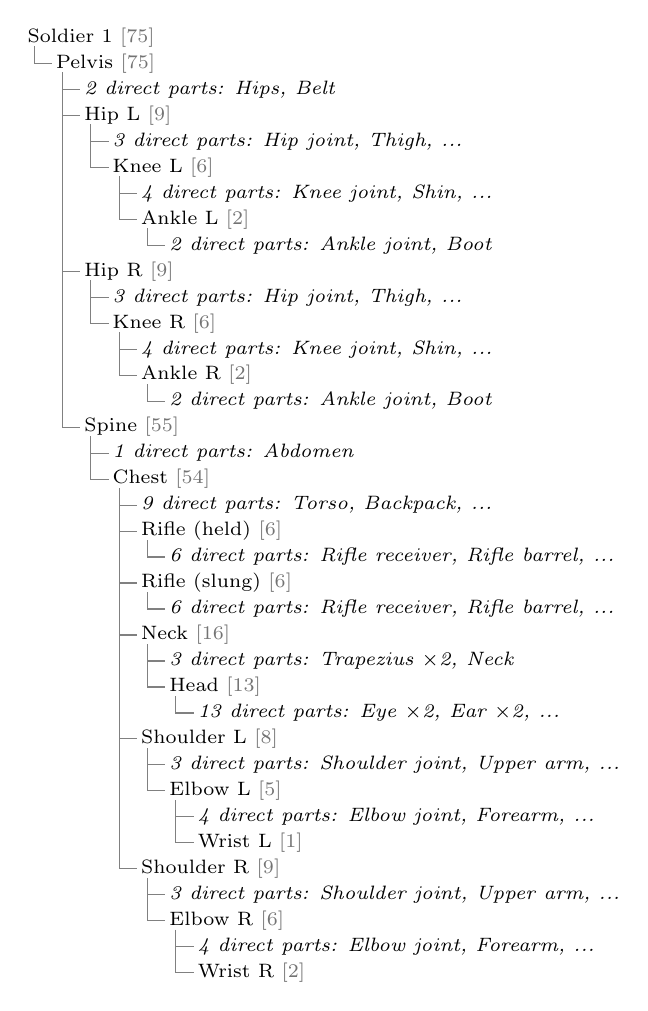
\begin{tikzpicture}[x=0.36cm,y=-0.33cm,font=\scriptsize]
\node[anchor=west,inner sep=0pt] (n0) at (0,0) {Soldier 1 \textcolor{black!55}{[75]}};
\node[anchor=west,inner sep=0pt] (n1) at (1,1) {Pelvis \textcolor{black!55}{[75]}};
\draw[black!50,thin] (0.25,0.35) |- (0.88,1);
\node[anchor=west,inner sep=0pt] (n2) at (2,2) {\textit{2 direct parts: Hips, Belt}};
\draw[black!50,thin] (1.25,1.35) |- (1.88,2);
\node[anchor=west,inner sep=0pt] (n3) at (2,3) {Hip L \textcolor{black!55}{[9]}};
\draw[black!50,thin] (1.25,1.35) |- (1.88,3);
\node[anchor=west,inner sep=0pt] (n4) at (3,4) {\textit{3 direct parts: Hip joint, Thigh, ...}};
\draw[black!50,thin] (2.25,3.35) |- (2.88,4);
\node[anchor=west,inner sep=0pt] (n5) at (3,5) {Knee L \textcolor{black!55}{[6]}};
\draw[black!50,thin] (2.25,3.35) |- (2.88,5);
\node[anchor=west,inner sep=0pt] (n6) at (4,6) {\textit{4 direct parts: Knee joint, Shin, ...}};
\draw[black!50,thin] (3.25,5.35) |- (3.88,6);
\node[anchor=west,inner sep=0pt] (n7) at (4,7) {Ankle L \textcolor{black!55}{[2]}};
\draw[black!50,thin] (3.25,5.35) |- (3.88,7);
\node[anchor=west,inner sep=0pt] (n8) at (5,8) {\textit{2 direct parts: Ankle joint, Boot}};
\draw[black!50,thin] (4.25,7.35) |- (4.88,8);
\node[anchor=west,inner sep=0pt] (n9) at (2,9) {Hip R \textcolor{black!55}{[9]}};
\draw[black!50,thin] (1.25,1.35) |- (1.88,9);
\node[anchor=west,inner sep=0pt] (n10) at (3,10) {\textit{3 direct parts: Hip joint, Thigh, ...}};
\draw[black!50,thin] (2.25,9.35) |- (2.88,10);
\node[anchor=west,inner sep=0pt] (n11) at (3,11) {Knee R \textcolor{black!55}{[6]}};
\draw[black!50,thin] (2.25,9.35) |- (2.88,11);
\node[anchor=west,inner sep=0pt] (n12) at (4,12) {\textit{4 direct parts: Knee joint, Shin, ...}};
\draw[black!50,thin] (3.25,11.35) |- (3.88,12);
\node[anchor=west,inner sep=0pt] (n13) at (4,13) {Ankle R \textcolor{black!55}{[2]}};
\draw[black!50,thin] (3.25,11.35) |- (3.88,13);
\node[anchor=west,inner sep=0pt] (n14) at (5,14) {\textit{2 direct parts: Ankle joint, Boot}};
\draw[black!50,thin] (4.25,13.35) |- (4.88,14);
\node[anchor=west,inner sep=0pt] (n15) at (2,15) {Spine \textcolor{black!55}{[55]}};
\draw[black!50,thin] (1.25,1.35) |- (1.88,15);
\node[anchor=west,inner sep=0pt] (n16) at (3,16) {\textit{1 direct parts: Abdomen}};
\draw[black!50,thin] (2.25,15.35) |- (2.88,16);
\node[anchor=west,inner sep=0pt] (n17) at (3,17) {Chest \textcolor{black!55}{[54]}};
\draw[black!50,thin] (2.25,15.35) |- (2.88,17);
\node[anchor=west,inner sep=0pt] (n18) at (4,18) {\textit{9 direct parts: Torso, Backpack, ...}};
\draw[black!50,thin] (3.25,17.35) |- (3.88,18);
\node[anchor=west,inner sep=0pt] (n19) at (4,19) {Rifle (held) \textcolor{black!55}{[6]}};
\draw[black!50,thin] (3.25,17.35) |- (3.88,19);
\node[anchor=west,inner sep=0pt] (n20) at (5,20) {\textit{6 direct parts: Rifle receiver, Rifle barrel, ...}};
\draw[black!50,thin] (4.25,19.35) |- (4.88,20);
\node[anchor=west,inner sep=0pt] (n21) at (4,21) {Rifle (slung) \textcolor{black!55}{[6]}};
\draw[black!50,thin] (3.25,17.35) |- (3.88,21);
\node[anchor=west,inner sep=0pt] (n22) at (5,22) {\textit{6 direct parts: Rifle receiver, Rifle barrel, ...}};
\draw[black!50,thin] (4.25,21.35) |- (4.88,22);
\node[anchor=west,inner sep=0pt] (n23) at (4,23) {Neck \textcolor{black!55}{[16]}};
\draw[black!50,thin] (3.25,17.35) |- (3.88,23);
\node[anchor=west,inner sep=0pt] (n24) at (5,24) {\textit{3 direct parts: Trapezius $\times$2, Neck}};
\draw[black!50,thin] (4.25,23.35) |- (4.88,24);
\node[anchor=west,inner sep=0pt] (n25) at (5,25) {Head \textcolor{black!55}{[13]}};
\draw[black!50,thin] (4.25,23.35) |- (4.88,25);
\node[anchor=west,inner sep=0pt] (n26) at (6,26) {\textit{13 direct parts: Eye $\times$2, Ear $\times$2, ...}};
\draw[black!50,thin] (5.25,25.35) |- (5.88,26);
\node[anchor=west,inner sep=0pt] (n27) at (4,27) {Shoulder L \textcolor{black!55}{[8]}};
\draw[black!50,thin] (3.25,17.35) |- (3.88,27);
\node[anchor=west,inner sep=0pt] (n28) at (5,28) {\textit{3 direct parts: Shoulder joint, Upper arm, ...}};
\draw[black!50,thin] (4.25,27.35) |- (4.88,28);
\node[anchor=west,inner sep=0pt] (n29) at (5,29) {Elbow L \textcolor{black!55}{[5]}};
\draw[black!50,thin] (4.25,27.35) |- (4.88,29);
\node[anchor=west,inner sep=0pt] (n30) at (6,30) {\textit{4 direct parts: Elbow joint, Forearm, ...}};
\draw[black!50,thin] (5.25,29.35) |- (5.88,30);
\node[anchor=west,inner sep=0pt] (n31) at (6,31) {Wrist L \textcolor{black!55}{[1]}};
\draw[black!50,thin] (5.25,29.35) |- (5.88,31);
\node[anchor=west,inner sep=0pt] (n32) at (4,32) {Shoulder R \textcolor{black!55}{[9]}};
\draw[black!50,thin] (3.25,17.35) |- (3.88,32);
\node[anchor=west,inner sep=0pt] (n33) at (5,33) {\textit{3 direct parts: Shoulder joint, Upper arm, ...}};
\draw[black!50,thin] (4.25,32.35) |- (4.88,33);
\node[anchor=west,inner sep=0pt] (n34) at (5,34) {Elbow R \textcolor{black!55}{[6]}};
\draw[black!50,thin] (4.25,32.35) |- (4.88,34);
\node[anchor=west,inner sep=0pt] (n35) at (6,35) {\textit{4 direct parts: Elbow joint, Forearm, ...}};
\draw[black!50,thin] (5.25,34.35) |- (5.88,35);
\node[anchor=west,inner sep=0pt] (n36) at (6,36) {Wrist R \textcolor{black!55}{[2]}};
\draw[black!50,thin] (5.25,34.35) |- (5.88,36);
\end{tikzpicture}
